\documentclass[a4paper,twoside]{article}
\usepackage{blindtext}  
\usepackage{geometry}

% Chinese support
\usepackage[UTF8, scheme = plain]{ctex}

% Page margin layout
\geometry{left=2.3cm,right=2cm,top=2.5cm,bottom=2.0cm}


\usepackage{listings}
\usepackage{xcolor}
\usepackage{geometry}
\usepackage{amsmath}
\usepackage{float}
\usepackage{hyperref}

\usepackage{graphics}
\usepackage{graphicx}
\usepackage{subcaption}
\usepackage{epsfig}
\usepackage{float}

\usepackage{algorithm}
\usepackage[noend]{algpseudocode}

\usepackage{booktabs}
\usepackage{threeparttable}
\usepackage{longtable}
\usepackage{tikz}
\usepackage{multicol}
\usepackage{pgfplots}
\pgfplotsset{compat=1.9}
\pgfplotsset{
    myplotstyle/.style={
    legend style={draw=none, font=\small},
    legend cell align=left,
    legend pos=north east,
    ylabel style={align=center, font=\bfseries\boldmath},
    xlabel style={align=center, font=\bfseries\boldmath},
    x tick label style={font=\bfseries\boldmath},
    y tick label style={font=\bfseries\boldmath},
    scaled ticks=false,
    every axis plot/.append style={thick},
    },
}

% cite package, to clean up citations in the main text. Do not remove.
\usepackage{cite}

\usepackage{color,xcolor}

%% The amssymb package provides various useful mathematical symbols
\usepackage{amssymb}
%% The amsthm package provides extended theorem environments
\usepackage{amsthm}
\usepackage{amsfonts}
\usepackage{enumerate}
\usepackage{enumitem}
\usepackage{listings}
\usepackage{minted}


\usepackage{indentfirst}
\setlength{\parindent}{2em} % Make two letter space in the first paragraph
\usepackage{setspace}
\linespread{1.5} % Line spacing setting
\usepackage{siunitx}
\setlength{\parskip}{0.5em} % Paragraph spacing setting

% \usepackage[contents =22920202204622, scale = 10, color = black, angle = 50, opacity = .10]{background}

\renewcommand{\figurename}{图}
\renewcommand{\listingscaption}{代码}
\renewcommand{\tablename}{表格}
\renewcommand{\contentsname}{目录}
\floatname{algorithm}{算法}

\graphicspath{ {images/} }

%%%%%%%%%%%%%
\newcommand{\StudentNumber}{22920202204622}  % Fill your student number here
\newcommand{\StudentName}{熊恪峥}  % Replace your name here
\newcommand{\PaperTitle}{实验(二)线程与同步}  % Change your paper title here
\newcommand{\PaperType}{操作系统实验报告} % Replace the type of your report here
\newcommand{\Date}{2023年4月19日}
\newcommand{\College}{信息学院}
\newcommand{\CourseName}{操作系统}
%%%%%%%%%%%%%

%% Page header and footer setting
\usepackage{fancyhdr}
\usepackage{lastpage}
\pagestyle{fancy}
\fancyhf{}
% This requires the document to be twoside
\fancyhead[LO]{\texttt{\StudentName }}
\fancyhead[LE]{\texttt{\StudentNumber}}
\fancyhead[C]{\texttt{\PaperTitle }}
\fancyhead[R]{\texttt{第{\thepage}页,共\pageref*{LastPage}页}}


\title{\PaperTitle}
\author{\StudentName}
\date{\Date}

\algnewcommand\algorithmicinput{\textbf{Input:}}
\algnewcommand\algorithmicoutput{\textbf{Output:}}
\algnewcommand\Input{\item[\algorithmicinput]}%
\algnewcommand\Output{\item[\algorithmicoutput]}%

\usetikzlibrary{positioning, shapes.geometric,arrows,automata}

\tikzstyle{startstop} = [rectangle, rounded corners, minimum width=3cm, minimum height=1cm, text centered, draw=black, fill=red!30]
\tikzstyle{io} = [trapezium, trapezium left angle=70, trapezium right angle=110, minimum width=3cm, minimum height=1cm, text centered, draw=black, fill=blue!30]
\tikzstyle{process} = [rectangle, minimum width=3cm, minimum height=1cm, text centered, draw=black, fill=green!30]
\tikzstyle{decision} = [diamond, minimum width=3cm, minimum height=1cm, text centered, draw=black, fill=yellow!30]
\tikzstyle{arrow} = [thick,->,>=stealth]

\begin{document}
	
%%%%%%%%%%%%%%%%%%%%%%%%%%%%%%%%%%%%%%%%%%%%
\makeatletter % change default title style
\renewcommand*\maketitle{%
	\begin{center} 
		\bfseries  % title 
		{\LARGE \@title \par}  % LARGE typesetting
		\vskip 1em  %  margin 1em
		{\global\let\author\@empty}  % no author information
		{\global\let\date\@empty}  % no date
		\thispagestyle{empty}   %  empty page style
	\end{center}%
	\setcounter{footnote}{0}%
}
\makeatother
%%%%%%%%%%%%%%%%%%%%%%%%%%%%%%%%%%%%%%%%%%%%
	
	
\thispagestyle{empty}

\vspace*{1cm}

\begin{figure}[htb]
	\centering
	
\includegraphics[width=4.0cm]{logo.png}
\end{figure}

\vspace*{1cm}

\begin{center}
	\Huge{\textbf{\PaperType}}
	
	\Large{\PaperTitle}
\end{center}

\vspace*{1cm}

\begin{table}[H]
	\centering	
	\begin{Large}
		\renewcommand{\arraystretch}{1.5}
		\begin{tabular}{p{3cm} p{5cm}<{\centering}}
			姓\qquad 名 & \StudentName  \\
			\hline
			学\qquad号 & \StudentNumber \\
			\hline
			日\qquad期 & \Date  \\
			\hline
			学\qquad院 & \College  \\
			\hline
			课程名称 & \CourseName  \\
			\hline
		\end{tabular}
	\end{Large}
\end{table}

\newpage

\title{
	\Large{\textcolor{black}{\PaperTitle}}
}

\maketitle
	
\tableofcontents
 
\newpage
\setcounter{page}{1}

\begin{spacing}{1.2}

\section{实现锁机制和条件变量}

\subsection{使用RAII确保正确互斥和正确的中断状态管理}

RAII(Resource Acquisition Is Initialization)是一种在C++编程中广泛使用的技术,
用于自动化管理资源的获取和释放。RAII的核心思想是,通过对象的构造函数获取资源,
通过对象的析构函数释放资源。这样可以避免资源泄漏和内存泄漏等常见的程序错误,
同时也使代码更加简洁、易于维护。

在并发编程中,锁是一种常见的同步机制,用于保护共享资源的访问。
手动管理锁的获取和释放可能会出现各种问题,如忘记释放锁等。并且即使代码中进行了正确的处理,
许多因素也可能导致正常的控制流被打断,进而导致不正确的行为。例如异常机制。

RAII技术可以用来更好地管理锁的获取和释放,避免这些常见的问题。
在C++标准库中,有\texttt{std::lock\_guard}
和\texttt{std::unique\_lock}等RAII类,
用于管理互斥锁和读写锁的获取和释放。在Nachos中,我首先根据给定的接口定义实现了功能类似的
\texttt{LockGuard}
和\texttt{InterruptScope}。
其中,\texttt{LockGuard}用于管理互斥锁的获取和释放,
\texttt{InterruptScope}用于自动管理中断状态的启用和关闭。
以\texttt{LockGuard}为例,实现如代码~\ref{code:lockguard}。

使用RAII来管理锁的获取和释放、以及中断的启用和关闭,Nachos可以确保在离开临界区时自动释放锁,
即使在临界区抛出异常或提前返回等情况下,锁也会被正确地释放,中断同理。

此外,RAII还可以使代码更加简洁、易于维护,用一种近似“声明式”的方法对各种资源进行管理,避免了业务逻辑中大量语法噪声的存在。

\begin{listing}[htb]
	\caption{\texttt{LockGuard}实现}
	\label{code:lockguard}
	\begin{minted}{cpp}
class LockGuard final {
public:
  LockGuard(Lock& lock):lock_(&lock) {
    lock_->Acquire();
  }
  
  LockGuard(Lock* lock):lock_(lock) {
    lock_->Acquire();
  }

  ~LockGuard()
  {
    lock_->Release();
  }
private:
  Lock* lock_;
};
	\end{minted}
\end{listing}

有了上述两个工具类,就可以更好地使用同步机制。因此,下面对具体的同步机制进行实现。

\subsection{使用\texttt{Thread::Sleep}实现锁机制和条件变量}

锁是一种基础的同步工具。锁的作用是保证只有一个进程可以访问被保护的共享资源。
在真实世界中最为常见的锁是自旋锁。对于某些较为简易的操作系统内核,例如\texttt{xv6},
自旋锁是提供的最主要的互斥机制。然而自旋锁也有诸多缺点,例如自旋等待消耗了大量的CPU时间,
使用\texttt{Thread::Sleep}实现锁,就可以将睡眠等待用作自选等待的替代,进而解决上述问题。

使用\texttt{Thread::Sleep}实现锁,其关键在于管理线程的睡眠和唤醒。因此重要工作就是对
休眠队列的维护:
\begin{itemize}
\item \texttt{Acquire}方法的实现锁的获取,如图~\ref*{fig:slpacq}。首先,当锁被占用时,线程会进入休眠队列并进入休眠状态。在获取锁时,需要确保获取锁的原子性,避免并发问题的发生。因此,这个实现中使用了禁用中断的机制来确保获取锁的原子性。
\item \texttt{Release}方法,如图~\ref*{fig:slprel},主要功能是释放锁,并将等待队列中的第一个线程唤醒。
在方法实现中,它首先判断当前线程是否持有该锁,如果不是则报错。
然后进行解锁操作,然后如果等待队列不为空,则将队列中的第一个线程取出,并将其放入就绪队列中。
\end{itemize}

\begin{figure}[h]
\centering
\caption{使用\texttt{Thread::Sleep}获取和释放锁}
\begin{subfigure}{0.4\textwidth}
	\centering
	\caption{使用\texttt{Thread::Sleep}获取锁}
	\label{fig:slpacq}
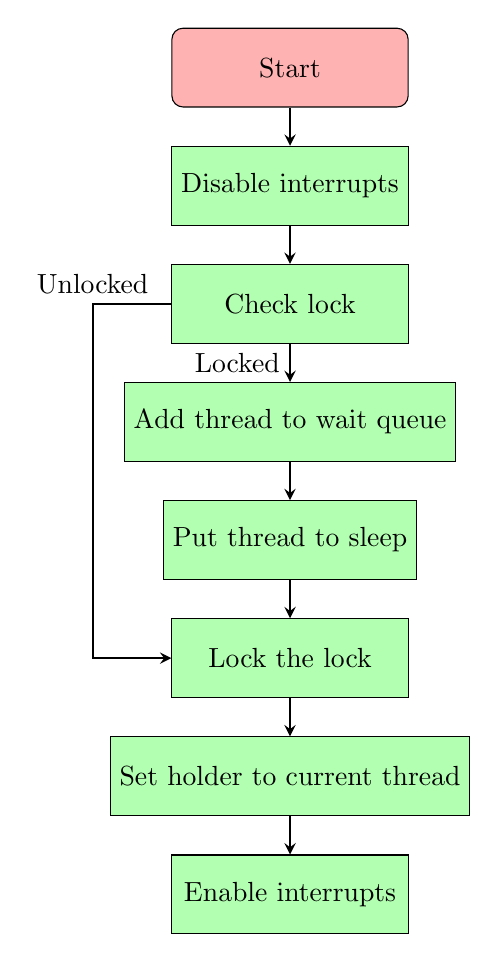
\begin{tikzpicture}[node distance=1.5cm]
	\node (start) [startstop] {Start};
	\node (acquire1) [process, below of=start] {Disable interrupts};
	\node (acquire2) [process, below of=acquire1] {Check lock};
	\node (acquire3) [process, below of=acquire2] {Add thread to wait queue};
	\node (acquire4) [process, below of=acquire3] {Put thread to sleep};
	\node (acquire5) [process, below of=acquire4] {Lock the lock};
	\node (acquire6) [process, below of=acquire5] {Set holder to current thread};
	\node (acquire7) [process, below of=acquire6] {Enable interrupts};

	\draw [arrow] (start) -- (acquire1);
	\draw [arrow] (acquire1) -- (acquire2);
	\draw [arrow] (acquire2) -- node[anchor=east] {Locked} (acquire3);
	\draw [arrow] (acquire2.west) -- ++(-1,0) node[anchor=south] {Unlocked} |- (acquire5.west);
	\draw [arrow] (acquire3) -- (acquire4);
	\draw [arrow] (acquire4) -- (acquire5);
	\draw [arrow] (acquire5) -- (acquire6);
	\draw [arrow] (acquire6) -- (acquire7);

\end{tikzpicture}
\end{subfigure}\begin{subfigure}{0.4\textwidth}
	\centering
	\caption{使用\texttt{Thread::Sleep}释放锁}
	\label{fig:slprel}
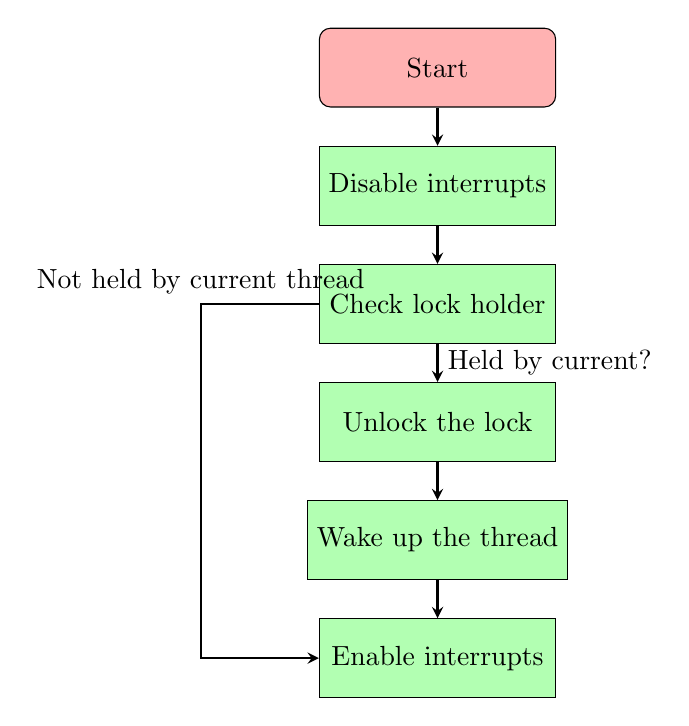
\begin{tikzpicture}[node distance=1.5cm]

	\node (start) [startstop] {Start};
	\node (disable) [process, below of=start] {Disable interrupts};
	\node (check) [process, below of=disable] {Check lock holder};
	\node (unlock) [process, below of=check] {Unlock the lock};
	\node (wake) [process, below of=unlock] {Wake up the thread};
	\node (enable) [process, below of=wake] {Enable interrupts};

	\draw [arrow] (start) -- (disable);
	\draw [arrow] (disable) -- (check);
	\draw [arrow] (check) -- node[anchor=west] {Held by current?} (unlock);
	\draw [arrow] (check.west) -- ++(-1.5,0) node[anchor=south] {Not held by current thread} |- (enable.west);
	\draw [arrow] (unlock) -- (wake);
	\draw [arrow] (wake) -- (enable);

\end{tikzpicture}
\end{subfigure}

\end{figure}


\subsection{使用\texttt{Semaphore}实现锁机制和条件变量}

锁在功能上相当于信号量的特殊情况,即只有一个资源的信号量,
但是锁限制释放和获取的必须是同一个线程。因此,使用信号量来实现锁,
可以分为两个部分:
\begin{enumerate}
	\item 使用二元信号量自动处理释放和获取,以及对休眠队列的维护。
	\item 检查获取和释放锁的线程是否相同。
\end{enumerate}
由于主要的互斥都由信号量保证,因此实现更加简单。以获取为例,实现如代码~\ref{code:semacq}。
\begin{listing}[H]
	\caption{获取锁的实现}
	\label{code:semacq}
	\begin{minted}{cpp}
InterruptScope cli(IntOff);
sem_.P();
locked_ = true;
owner_ = currentThread;
	\end{minted}
\end{listing}

与使用\texttt{Thread::Sleep}相比,这个实现更为简洁。需要注意的是,不应当忘记关闭中断。

\subsection{用锁机制和条件变量修改双向有序链表}

使用锁和条件变量修改双向有序链表,只需要为链表整体加锁。因为链表在空间上理论不受限,所以不需要通过管程等结构
限制大小。例如在头部插入的函数加锁后如代码~\ref{code:append},利用\texttt{LockGuard}实现只需要一行
即可完成加锁。

\begin{listing}[htb]
	\caption{插入实现}
	\label{code:append}
	\begin{minted}{cpp}
void DLList::Append(void* item)
{
	LockGuard g(lock_); // 新增代码

	RAIIListValidator _(*this, __FUNCTION__);

	DLLElement* element = new DLLElement(item, 0);

	if (!IsEmpty())		// list is empty
	{
		first = last = element;
	}
	else				// otherwise
	{
		element->key = last->key + 1;
		element->prev = last;
		last->next = element;
		last = element;
	}

	condvar_->Signal(lock_);
}
	\end{minted}
\end{listing}

\emph{需要注意的是,不仅修改操作需要加锁,任何访问链接结构的代码都需要加锁。}

这是因为,在遍历、读取链表节点的过程中要求链表具有完整的结构,此时修改的线程可能在修改途中,而使得
链表的结构不完整。例如有未设置完成的指针。

一方面,可以把该问题设计为一个读者写者问题,即读取链表元素、遍历链表等操作的线程为读者,修改链表的线程为写者。但是这样的实现较为复杂。
实际上,只要保证访问链表的所有过程完全互斥,也可以保证线程安全。

另一方面,某些操作需要链表非空时才能完成,例如\texttt{Remove}等。为了解决这一问题,可以利用管程。使用条件变量来完成对非空条件的等待。
例如\texttt{Remove}如的一段节选如代码~\ref{code:remove},它在\texttt{empty\_}上等待,直到不空为止。而那些插入操作在完成后,会唤醒等待的线程。
例如代码~\ref{code:append}以对条件变量的\texttt{Signal}操作结束,它会使得一个等待不为空的线程被唤醒。
\begin{listing}[H]
	\caption{Remove的部分实现}
	\label{code:remove}
	\begin{minted}{cpp}
void* DLList::Remove(int* keyPtr)
{
	...
	while (IsEmpty())
		condvar_->Wait(lock_);	
	...
}
	\end{minted}
\end{listing}

\subsection{测试}

为了测试,线程安全的双线链表实现,我使用了实验一中的代码。作为快速的回忆,在实验一中,
我实现了基于\texttt{RAII}的链表自动检查,来检查链表中可能出现的错误。

如图~\ref{fig:threads},在实验一中观察到不当设置指针导致的Segmentation Fault错误的位置\texttt{Yield}也不会导致任何问题的产生。
因为它通过了自动检查器的检查。

\begin{figure}[htb]
	\centering
	\caption{线程安全的双向链表测试}
	\label{fig:threads}
	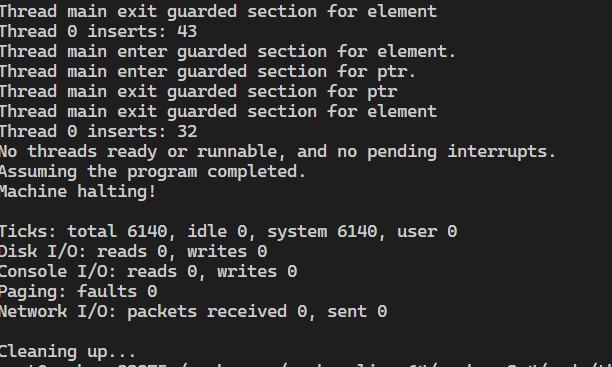
\includegraphics[width=0.6\linewidth]{thread.png}
\end{figure}

\newpage

\section{实现一个线程安全的表结构}

实验要求实现一个线程安全的表结构。为了保证线程安全,需要使用锁机制来保证同一时间只能有一个线程访问表。

在实现中,Table类包含了表结构的大小、表项的指针数组以及一个锁对象。构造函数初始化了指针数组和锁对象,析构函数负责释放指针数组和锁对象的内存。

表结构的操作包括Alloc、Get和Release三个方法,分别用于分配表项、获取表项和释放表项。其中Alloc方法需要遍历指针数组,找到第一个未被使用的表项,并将其分配给对象。
Get和Release方法只需要简单地获取或释放表项的指针即可。

为了保证线程安全,这里的策略也是使用锁来保证方法级的互斥。
在每个方法中都使用了LockGuard类来获取和释放锁,
保证了锁的自动释放,避免了手动管理锁带来的不便和风险。这是因为
这个类的使用并不会出现任何的经典互斥问题,例如“读者写者问题”、“生产者消费者问题”等。

以分配和回收为例,它们的实现如代码~\ref{code:allocrelase}。
\begin{listing}[htb]
	\caption{分配和回收的实现}
	\label{code:allocrelase}
	\begin{minted}{cpp}
int Table::Alloc(void *object)
{
    LockGuard _(lock_);
    for (int i = 0;i < size_;i++)
    {
        if (!items_[i])
        {
            items_[i] = object;
            return i;
        }
    }
    return -1;
}
void Table::Release(int index)
{
    LockGuard _(lock_);
    items_[index] = NULL;
}
	\end{minted}
\end{listing}

\subsection{测试}

其运行结果如图~\ref{fig:tbl}。可见多个线程可以正常地进行存取。
\begin{figure}[htb]
	\centering
	\caption{线程安全的表结构测试}
	\label{fig:tbl}
	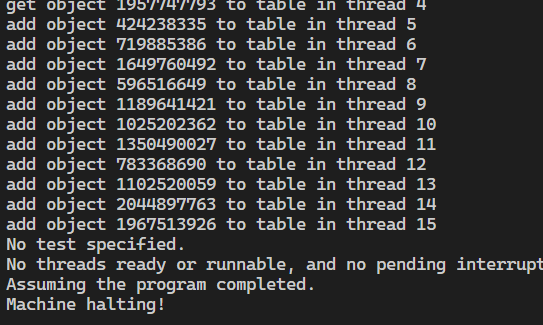
\includegraphics[width=0.4\linewidth]{tbl.png}
\end{figure}


\newpage

\section{实现一个大小受限的缓冲区}

有界缓冲区有两个主要的方法,分别是写方法\texttt{Write}和读方法\texttt{Read}。
使用缓冲区的过程,实质上就是一个缓冲区大小受限的生产者消费者问题。因此为了保证线程安全,
我在类中使用了锁以及条件变量,进而使用管程的结构保证正确的执行。

在管程解决生产者消费者问题的基本框架下,实际的业务逻辑就是维护循环队列的队头元素、队尾元素的索引。
因此,将业务逻辑置于管程解决生产者消费者问题的框架下,就得到了具体实现,如代码~\ref{code:buf}。

\begin{listing}[htb]
	\caption{\texttt{BoundedBuffer}实现}
	\label{code:buf}
	\begin{minted}{cpp}
void BoundedBuffer::Write(void* data, int size) {
    LockGuard g(mutex_);
    while (!(size_ < maxsize_))
    {
        not_full_->Wait(mutex_);
    }
    char* data_ptr = (char*)(data);
    for (int i = 0; i < size; i++) {
        buffer_[tail_] = data_ptr[i];
        tail_ = (tail_ + 1) % maxsize_;
        size_++;
    }
    not_empty_->Broadcast(mutex_);
}
void BoundedBuffer::Read(void* data, int size) {
    LockGuard g(mutex_);
    while (!(size_ >= size))
    {
        not_empty_->Wait(mutex_);
    }
    char* data_ptr = (char*)(data);
    for (int i = 0; i < size; i++) {
        data_ptr[i] = buffer_[head_];
        head_ = (head_ + 1) % maxsize_;
        size_--;
    }
    not_full_->Broadcast(mutex_);
}
	\end{minted}
\end{listing}

\subsection{测试}

运行效果如图~\ref{fig:buf}。线程1负责生产15个元素,其余的线程分别获得$pid-1$个元素。
可见,线程安全的缓冲区可以正常地工作。并且想要获得超过15个的额外元素的线程被置于休眠模式了。
\begin{figure}[H]
	\centering
	\caption{线程安全的缓冲区测试}
	\label{fig:buf}
	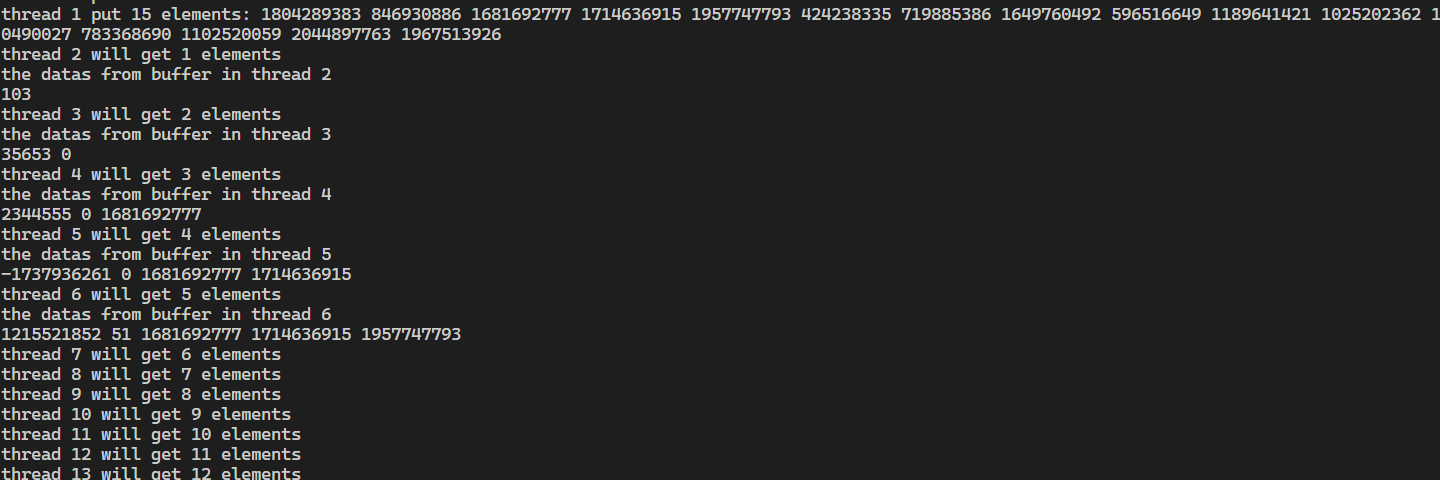
\includegraphics[width=0.6\linewidth]{bb.png}
\end{figure}

\newpage

\section{实验总结}


本次实验让我深入了解了操作系统中同步机制的实现和原理,通过手动实现锁和条件变量,我对这些机制的工作流程和应用场景有了更深刻的认识。同时,我也学习了如何使用这些同步机制来保证多线程程序的正确性和可靠性,以及如何在实践中避免常见的并发错误。在实现线程安全的双向有序链表和表结构时,我了解到不同同步机制的应用场景和使用方法,对于如何在多个线程之间实现数据共享和访问,我有了更加全面的认识。在实现大小受限的缓冲区时,我体会到了同步机制的重要性,只有正确地使用锁和条件变量,才能确保程序的正确性和稳定性。通过这次实验,我掌握了操作系统中同步机制的基本原理和使用方法,对于编写高效、可靠的多线程程序有了更加深入的了解。

在本次实验中,我成功实现了LockGuard类,并使用它来自动管理锁。在实现过程中,我注意到需要重写之前的代码来适配LockGuard的使用,即把原先手动加锁和释放锁的代码改成使用LockGuard来管理锁。通过使用LockGuard,我可以避免忘记手动释放锁而导致的死锁问题,并且代码更加简洁,易于维护。

\end{spacing}

\end{document}